\documentclass[aspectratio=169, 11pt]{beamer}

% ========== 主题设置 ==========
\usetheme{Madrid}
\usecolortheme{whale}
\setbeamertemplate{navigation symbols}{}
\setbeamertemplate{footline}[frame number]

% ========== 包 ==========
\usepackage{tikz}
\usetikzlibrary{arrows.meta, positioning, shapes.geometric, calc, fit, backgrounds}
\usepackage{booktabs}
\usepackage{graphicx}
\usepackage{amsmath}
\usepackage{xcolor}

% ========== 颜色定义 ==========
\definecolor{highlight}{RGB}{255, 100, 100}
\definecolor{completed}{RGB}{100, 200, 100}
\definecolor{pending}{RGB}{200, 200, 200}
\definecolor{inprogress}{RGB}{100, 150, 255}

% ========== 标题信息 ==========
\title{Weekly Progress Report}
\subtitle{Week of Feb 11: PhysioNet Integration \& 3-Dataset RL Control}
\author{Student ID: 11314389}
\institute{BCI Control System Project}
\date{February 11, 2026}

\begin{document}

% ========== 标题页 ==========
\begin{frame}
    \titlepage
\end{frame}

% ========== Slide 1: 系统架构图 ==========
\begin{frame}{System Overview: Current Focus}
    \begin{center}
    \resizebox{0.95\textwidth}{!}{%
    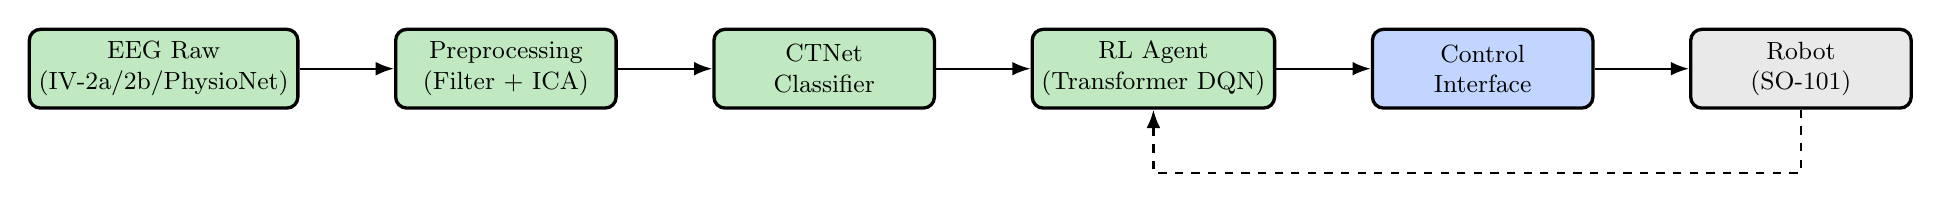
\begin{tikzpicture}[
        node distance=8mm and 12mm,
        block/.style={rectangle, rounded corners, draw, very thick,
                      minimum width=28mm, minimum height=10mm,
                      align=center, font=\small},
        arrow/.style={-Latex, thick},
    ]
        \node[block, fill=completed!40] (raw) {EEG Raw\\(IV-2a/2b/PhysioNet)};
        \node[block, fill=completed!40, right=of raw] (prep) {Preprocessing\\(Filter + ICA)};
        \node[block, fill=completed!40, right=of prep] (csp) {CTNet\\Classifier};
        \node[block, fill=completed!40, right=of csp] (dqn) {RL Agent\\(Transformer DQN)};
        \node[block, fill=inprogress!40, right=of dqn] (ctrl) {Control\\Interface};
        \node[block, fill=pending!40, right=of ctrl] (robot) {Robot\\(SO-101)};
        
        \draw[arrow] (raw) -- (prep);
        \draw[arrow] (prep) -- (csp);
        \draw[arrow] (csp) -- (dqn);
        \draw[arrow] (dqn) -- (ctrl);
        \draw[arrow] (ctrl) -- (robot);
        
        \draw[arrow, dashed] (robot.south) -- ++(0,-8mm) -| (dqn.south);
        
    \end{tikzpicture}}
    \end{center}
    
    \vspace{3mm}
    \begin{columns}[T]
        \column{0.5\textwidth}
        \textbf{Legend:}
        \begin{itemize}
            \item[\textcolor{completed}{\rule{8pt}{8pt}}] Completed
            \item[\textcolor{inprogress}{\rule{8pt}{8pt}}] In Progress
        \end{itemize}
        \column{0.5\textwidth}
        \begin{itemize}
            \item[\textcolor{highlight}{\rule{8pt}{8pt}}] This Week's Focus
            \item[\textcolor{pending}{\rule{8pt}{8pt}}] Pending
        \end{itemize}
    \end{columns}
\end{frame}

% ========== Slide 2: 本周目标 ==========
\begin{frame}{This Week's Goals}
    \begin{enumerate}
        \item \textbf{Integrate Third Dataset: PhysioNet EEGMMIDB}
        \begin{itemize}
            \item 109 subjects, 64 channels, 160 Hz
            \item Left/right hand motor imagery tasks
        \end{itemize}
        
        \vspace{3mm}
        \item \textbf{CTNet Classification Test on PhysioNet}
        \begin{itemize}
            \item Validate classification performance on new dataset
        \end{itemize}
        
        \vspace{3mm}
        \item \textbf{3-Dataset RL Control Comparison}
        \begin{itemize}
            \item IV-2a (22ch, 4-class) vs IV-2b (3ch, 2-class) vs PhysioNet (64ch, 2-class)
            \item Evaluate control reach rate and trajectory smoothness
        \end{itemize}
    \end{enumerate}
\end{frame}

% ========== Slide 3: 方法 ==========
\begin{frame}{Methods: PhysioNet Dataset Integration}
    \textbf{PhysioNet EEG Motor Movement/Imagery Dataset}
    \begin{itemize}
        \item \textbf{Source:} \url{https://physionet.org/content/eegmmidb/1.0.0/}
        \item \textbf{Subjects:} 109 (vs 9 in IV-2a/2b)
        \item \textbf{Channels:} 64 (10-10 system)
        \item \textbf{Tasks:} Real/imagined left-right hand, both fists/feet
        \item \textbf{Format:} EDF+ (loaded via MNE-Python)
    \end{itemize}
    
    \vspace{3mm}
    \textbf{Data Pipeline:}
    \begin{enumerate}
        \item Download per-subject EDF files (supports partial download)
        \item Load with MNE, extract motor imagery runs (4, 8, 12)
        \item Apply 8-30 Hz bandpass filter
        \item Split train/test (80/20)
    \end{enumerate}
\end{frame}

% ========== Slide 4: 结果 - 分类 ==========
\begin{frame}{Results: CTNet Classification (3 Subjects)}
    \begin{center}
    \begin{tabular}{lccc}
        \toprule
        \textbf{Dataset} & \textbf{Channels} & \textbf{Classes} & \textbf{Accuracy} \\
        \midrule
        IV-2a & 22 & 4 & 63.19\% \\
        IV-2b & 3 & 2 & 65.64\% \\
        \textbf{PhysioNet} & \textbf{64} & \textbf{2} & \textbf{70.37\%} \\
        \bottomrule
    \end{tabular}
    \end{center}
    
    \vspace{5mm}
    \textbf{Observations:}
    \begin{itemize}
        \item PhysioNet achieves highest classification accuracy (70.37\%)
        \item 64-channel montage provides richer spatial information
        \item Binary classification (L/R) is easier than 4-class
    \end{itemize}
\end{frame}

% ========== Slide 5: 结果 - RL控制 ==========
\begin{frame}{Results: RL Control Performance}
    \begin{center}
    \begin{tabular}{lccc}
        \toprule
        \textbf{Dataset} & \textbf{Classification} & \textbf{Control Rate} & \textbf{Smoothness} \\
        \midrule
        IV-2a & 63.19\% & \textcolor{green!60!black}{\textbf{99.33\%}} & 0.700 \\
        IV-2b & 65.64\% & \textcolor{green!60!black}{\textbf{98.00\%}} & 0.672 \\
        PhysioNet & 70.37\% & \textcolor{green!60!black}{\textbf{99.00\%}} & 0.681 \\
        \bottomrule
    \end{tabular}
    \end{center}
    
    \vspace{5mm}
    \textbf{Key Finding:}
    \begin{itemize}
        \item \textbf{RL control achieves 98-99\% reach rate across ALL datasets!}
        \item Classification accuracy $\neq$ Control success
        \item RL agent compensates for classification errors via temporal integration
        \item Consistent trajectory smoothness ($\sim$0.68-0.70)
    \end{itemize}
\end{frame}

% ========== Slide 6: 数据集对比图 ==========
\begin{frame}{Results: 3-Dataset Comparison Visualization}
    \begin{center}
    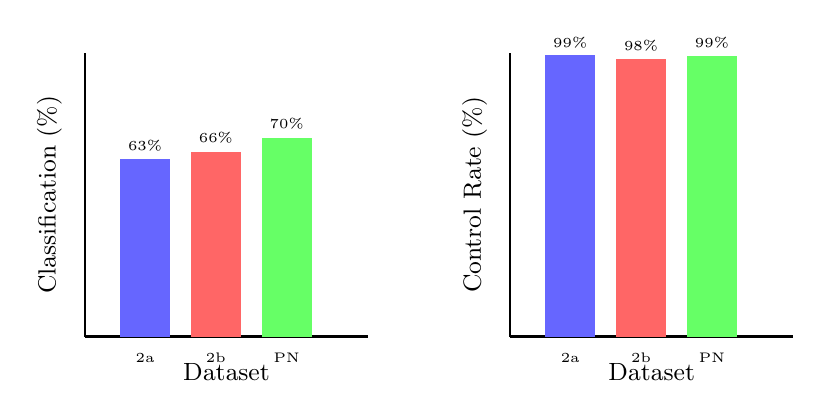
\begin{tikzpicture}[scale=0.9]
        % Classification Accuracy
        \draw[thick] (0,0) -- (0,4);
        \draw[thick] (0,0) -- (4,0);
        \node[rotate=90] at (-0.5,2) {\small Classification (\%)};
        \node at (2,-0.5) {\small Dataset};
        
        \fill[blue!60] (0.5,0) rectangle (1.2,2.5);  % IV-2a 63%
        \fill[red!60] (1.5,0) rectangle (2.2,2.6);   % IV-2b 66%
        \fill[green!60] (2.5,0) rectangle (3.2,2.8); % PhysioNet 70%
        
        \node at (0.85,-0.3) {\tiny 2a};
        \node at (1.85,-0.3) {\tiny 2b};
        \node at (2.85,-0.3) {\tiny PN};
        
        \node at (0.85,2.7) {\tiny 63\%};
        \node at (1.85,2.8) {\tiny 66\%};
        \node at (2.85,3.0) {\tiny 70\%};
        
        % Control Rate
        \begin{scope}[xshift=6cm]
        \draw[thick] (0,0) -- (0,4);
        \draw[thick] (0,0) -- (4,0);
        \node[rotate=90] at (-0.5,2) {\small Control Rate (\%)};
        \node at (2,-0.5) {\small Dataset};
        
        \fill[blue!60] (0.5,0) rectangle (1.2,3.97);  % IV-2a 99.3%
        \fill[red!60] (1.5,0) rectangle (2.2,3.92);   % IV-2b 98%
        \fill[green!60] (2.5,0) rectangle (3.2,3.96); % PhysioNet 99%
        
        \node at (0.85,-0.3) {\tiny 2a};
        \node at (1.85,-0.3) {\tiny 2b};
        \node at (2.85,-0.3) {\tiny PN};
        
        \node at (0.85,4.15) {\tiny 99\%};
        \node at (1.85,4.1) {\tiny 98\%};
        \node at (2.85,4.15) {\tiny 99\%};
        \end{scope}
    \end{tikzpicture}
    \end{center}
    
    \textbf{Conclusion:} RL control is robust across all three datasets with diverse characteristics!
\end{frame}

% ========== Slide 7: 挑战与解决 ==========
\begin{frame}{Challenges \& Solutions}
    \begin{columns}[T]
        \column{0.5\textwidth}
        \textbf{Challenges:}
        \begin{itemize}
            \item GigaScience dataset too large (226 GB)
            \item Different data formats (MAT vs EDF)
            \item PhysioNet label encoding differs
        \end{itemize}
        
        \column{0.5\textwidth}
        \textbf{Solutions:}
        \begin{itemize}
            \item Switched to PhysioNet (3.4 GB, per-subject download)
            \item Created unified loader with MNE
            \item Auto-detect label range in classifier
        \end{itemize}
    \end{columns}
    
    \vspace{5mm}
    \textbf{Code Structure:}
    \begin{itemize}
        \item \texttt{download\_physionet.py} - Download per-subject data
        \item \texttt{physionet\_loader.py} - Load and preprocess EDF files
        \item \texttt{rl\_control\_test.py} - Multi-dataset RL testing
    \end{itemize}
\end{frame}

% ========== Slide 8: 下一步 ==========
\begin{frame}{Next Steps}
    \begin{enumerate}
        \item \textbf{Controller/Limiter} (Priority)
        \begin{itemize}
            \item Add joint limit protection for robotic arm
            \item Prevent over-extension and collisions
        \end{itemize}
        
        \vspace{3mm}
        \item \textbf{Smoother + Delay}
        \begin{itemize}
            \item Reduce high-frequency oscillations in control
            \item Add interpolation between commands
        \end{itemize}
        
        \vspace{3mm}
        \item \textbf{Expand Subject Pool}
        \begin{itemize}
            \item Download more PhysioNet subjects (10-20)
            \item Report mean $\pm$ std across larger population
        \end{itemize}
        
        \vspace{3mm}
        \item \textbf{Physical Robot Testing}
        \begin{itemize}
            \item Deploy to SO-101 arm
            \item Real-time EEG $\rightarrow$ control pipeline
        \end{itemize}
    \end{enumerate}
\end{frame}

% ========== Slide 9: 时间线 ==========
\begin{frame}{Project Timeline}
    \begin{center}
    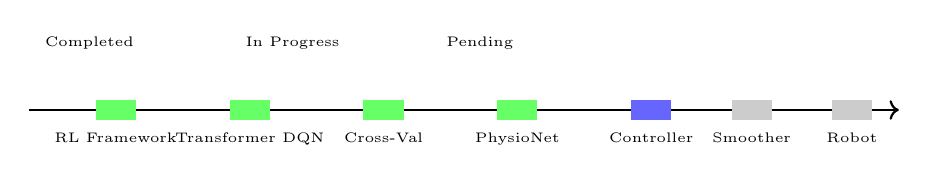
\begin{tikzpicture}[scale=0.85]
        \draw[thick, ->] (0,0) -- (13,0);
        
        % 已完成
        \foreach \x/\label in {1/RL Framework, 3/Transformer DQN, 5/Cross-Val, 7/PhysioNet} {
            \fill[green!60] (\x,-0.15) rectangle (\x+0.6,0.15);
            \node[below, font=\tiny] at (\x+0.3,-0.2) {\label};
        }
        
        % 进行中
        \fill[blue!60] (9,-0.15) rectangle (9.6,0.15);
        \node[below, font=\tiny] at (9.3,-0.2) {Controller};
        
        % 待完成
        \foreach \x/\label in {10.5/Smoother, 12/Robot} {
            \fill[gray!40] (\x,-0.15) rectangle (\x+0.6,0.15);
            \node[below, font=\tiny] at (\x+0.3,-0.2) {\label};
        }
        
        % 图例
        \node[right] at (0,1) {\tiny \textcolor{green!60!black}{$\blacksquare$} Completed};
        \node[right] at (3,1) {\tiny \textcolor{blue!60!black}{$\blacksquare$} In Progress};
        \node[right] at (6,1) {\tiny \textcolor{gray}{$\blacksquare$} Pending};
    \end{tikzpicture}
    \end{center}
    
    \vspace{5mm}
    \textbf{Summary:}
    \begin{itemize}
        \item Core RL pipeline complete with 3-dataset validation
        \item Next focus: Hardware interface and control refinement
    \end{itemize}
\end{frame}

% ========== 结束页 ==========
\begin{frame}
    \begin{center}
        \Huge Thank You!
        
        \vspace{10mm}
        \Large Questions?
    \end{center}
\end{frame}

\end{document}


